

%% Based on a TeXnicCenter-Template by Gyorgy SZEIDL.
%%%%%%%%%%%%%%%%%%%%%%%%%%%%%%%%%%%%%%%%%%%%%%%%%%%%%%%%%%%%%
%----------------------------------------------------------
%
\documentclass[11pt,a4paper,oneside,dutch,english]{book}

%
%
%----------------------------------------------------------
%%%%%%%%%%%%%%%%%%%%%%%%%%
%% PACKAGE LOADING TIME %%
%%%%%%%%%%%%%%%%%%%%%%%%%%
\usepackage{amsmath} 
\usepackage{amsfonts} 
\usepackage{amssymb} 
\usepackage{graphicx} 
\usepackage{subfigure} 
\usepackage{float}

%%--custom packages----------------------------------------
\usepackage{times} 
\usepackage[times]{quotchap} 
\usepackage[a4paper,verbose, asymmetric, centering]{geometry} 
\usepackage{url} 
\usepackage{flafter} 
\usepackage{todonotes} 
\usepackage[colorlinks=true, linkcolor=black, urlcolor=blue]{hyperref}

%----------------------------------------------------------
\newtheorem{theorem}{Theorem} 
\newtheorem{acknowledgement}[theorem]{Acknowledgement} 
\newtheorem{algorithm}[theorem]{Algorithm} 
\newtheorem{axiom}[theorem]{Axiom} 
\newtheorem{case}[theorem]{Case} 
\newtheorem{claim}[theorem]{Claim} 
\newtheorem{conclusion}[theorem]{Conclusion} 
\newtheorem{condition}[theorem]{Condition} 
\newtheorem{conjecture}[theorem]{Conjecture} 
\newtheorem{corollary}[theorem]{Corollary} 
\newtheorem{criterion}[theorem]{Criterion} 
\newtheorem{definition}[theorem]{Definition} 
\newtheorem{example}[theorem]{Example} 
\newtheorem{exercise}[theorem]{Exercise} 
\newtheorem{lemma}[theorem]{Lemma} 
\newtheorem{notation}[theorem]{Notation} 
\newtheorem{problem}[theorem]{Problem} 
\newtheorem{proposition}[theorem]{Proposition} 
\newtheorem{remark}[theorem]{Remark} 
\newtheorem{solution}[theorem]{Solution} 
\newtheorem{summary}[theorem]{Summary} 
\newenvironment{proof}[1][Proof]{\textbf{#1.} }{\ \rule{0.5em}{0.5em}} 
\newcommand{\npar}{\par \vspace{2.3ex plus 0.3ex minus 0.3ex} 
\noindent} 

% Om witruimte te krijgen tussen paragrafen
%%%%%%%%%%%%%%%%%%%%
%%  START BOOK    %%
%%%%%%%%%%%%%%%%%%%%
\begin{document}

\graphicspath{{images/}}

\frontmatter

%  Titelblad
\begin{titlepage}
	
	\fontsize{12pt}{14pt}\selectfont 
	\begin{center}
		\begin{figure}
			[H] 
			\begin{center}
				
\includegraphics[width=3cm, height=4cm]{VIB.pdf} \hfill 
				
\includegraphics{ugent.pdf} 
				\vfill 
				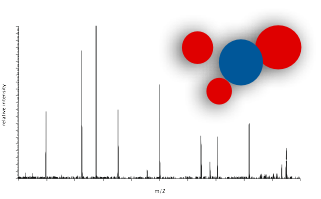
\includegraphics{mslims_logo.png} 
			\end{center}
		\end{figure}
		
		\vspace{0.3cm} 
		\begin{minipage}
			[c][4.5cm][c]{15cm} 
			\begin{center}
				\fontsize{22}{25pt}\selectfont {\textsc{ms-lims manual}} 
				\fontseries{m} \vspace{0.2cm} 
				\fontsize{12pt}{14pt}\selectfont \linebreak Kenny Helsens \linebreak Niklaas Colaert \linebreak Steffi Wortelkamp \linebreak Harald Barsnes \linebreak Marc Vaudel \linebreak Lennart Martens 
			\end{center}
		\end{minipage}
		
		\vspace{0.3cm}
		
		\vspace{0.8cm} Proteomics and Bioinformatics group \linebreak Departement of Medical Protein Research \linebreak VIB and Faculty of Medicine and Health Sciences, Ghent University \vspace{1cm} \linebreak
		
		\date \url{http://ms-lims.googlecode.com/} 
	\end{center}
\end{titlepage}

\tableofcontents

\listoftodos

\chapter{Introduction} 
\section*{Proteomics lims suite} \npar Mass spectrometry based proteomics approaches produce large amounts of mass spectra that require processing, identification and possibly quantification before interpretation can be undertaken. High-throughput studies require automation of these various steps, as well as management of the data in association with the results obtained. We here present ms-lims, a freely available, open-source system based on a central database to automate data management and processing in mass spectrometry driven proteomics analyses. \npar ms-lims is mainly designed to automate data flow in the high-throughput proteomics lab. Taking spectrum files from a variety of \emph{pluggable} fileformats (standard Micromass PKL file and Mascot Generic File support is provided), it transforms these to the Mascot Generic Format and stores them in the database, retaining LC information if present, and also allowing additional information to be stored for each individual LC run. Another part allows the retrieval of the stored spectra in mergefiles of arbitrary size. These can then be submitted to a search engine, eg. \emph{Mascot} from \emph{Matrix Science}. Subsequently, the results of these searches can be parsed and stored in a relational database structure for future reference. \npar ms-lims requires Java version 1.5 or above, which you can get from \url{http://java.com/}. Furthermore, ms-lims requires a running MySQL server which you can download freely from \url{http://www.mysql.com/downloads/mysql/}. Finally, download the ms-lims binaries from \url{http://ms-lims.googlecode.com} to get started with ms-lims. \npar The first part of this manual covers the installation, while the second part explains the actual tools of ms-lims 

\mainmatter

\part{Installation} 
\chapter{General} The installation of ms-lims cannot be done by a single installer but requires three consequent steps: 
\begin{description}
	\item[One] covers the installation of a Java Runtime Environment(JRE). Ms-lims was created with Java Development Kit(JDK) 1.5 and therefore needs a JRE starting version 1.5 (also known as Java 5) or later. 
	\item[Two] \textit{(shortly)} covers the installation of a database system. Ms-lims works around a central Relational Database Management System (RDBMS) to control the proteomics data. By preference, the freely available open source MySQL RDBMS is used for storage and manipulation of the proteomics data. 
	\item[Three] covers the installation of ms-lims itself. 
\end{description}

%% Chapter on Java installation.
%%%%%%%%%%%%%%%%%%%%%%%%%%%%%%%%
\chapter{Java}\label{Java} Since ms-lims was developed in Java, it runs on every operating system that has an up-to-date Java installation. It is highly probable that Java is already installed on your computer due to the widespread use of Java nowadays. Yet, if needed, a new Java installation is quite straightforward. 
\begin{itemize}
	\item Goto \url{http://java.com} 
	\item Follow the main download link and download the installer 
	\item When finished, open the installer and follow the instructions 
\end{itemize}
Java should be properly installed by now. Proceed to the next step.

%% Chapter on MySQL installation.
%%%%%%%%%%%%%%%%%%%%%%%%%%%%%%%%%%
\chapter{Relational Database Management System (RDBMS)}\label{RDBMS}

%% RDBMS
\section{Why a RDBMS?} 
\begin{quote}
	A short definition of a RDBMS may be a DBMS in which data is stored in the form of tables and the relationship among the data is also stored in the form of tables.\\\emph{Wikipedia} 
\end{quote}
\npar As for a proteomics oriented lims, whether you want to store fragmentation spectra or retrieve peptide identifications - the relation must be saved between the fragmentation spectrum and its peptide identifications. At all times, the relational database has a central role in the ms-lims for storing, managing and delivering this proteomics data. \npar Multiple RDMBS systems are availlable: MySQL, Oracle, Firebird, PostgreSQL, MS SQL Server are the most common examples. Even though there are all distinct RDBMS, they are similar as they are all SQL implementations. SQL means Structured Query Language and serves as a language for humans to communicate to the database holding all the proteomics data. All of these SQL implementing databases can be used with ms-lims by using different drivers. Hence, some of these are commercial while other are free open-source driven efforts. We prefer to use the popular open source database \textbf{MySQL} by default and will therefore orient this manual towards this database.

%%MYSQL
\section{MySQL} 
\subsection*{About MySQL} 
\begin{quote}
	The MySQL� RDBMS has become the world's most popular open source database because of its consistent fast performance, high reliability and ease of use.\\\emph{mysql.com} 
\end{quote}
For this reason amongst others, the developers of the lims system have chosen MySQL as the RDMBS of preference. A list of short instructions on the installation of MySQL follows. 
\subsection*{Getting MySQL} First, we will download the installer from the MySQL website. 
\begin{itemize}
	\item Goto the MySQL website at \url{http://mysql.com} 
	\item Click on the \textbf{download} tab in the top 
	\item Choose the \textbf{MySQL community server }to continue 
	\item Select the essential installer of your operating system and download it by the link at the right 
\end{itemize}
After downloading has finished, proceed to the installation.

\subsection*{Installing MySQL} 
\begin{itemize}
	\item Open the installer 
	\item Select the typical installation and proceed 
	\item Click the install button to start the installation of the MySQL server 
	\item Wait for the installation to complete. After completion, enable the \textbf{configure now} checkbox and to proceed to configure the database 
\end{itemize}
Now the installation has completed, the MySQL database needs some extra configurations regarding performance and security. 
\subsection*{Configuring MySQL} 
\begin{itemize}
	\item Verify you are now in the configuration window titled \textbf{'MySQL server instance configuration wizard'} 
	\item Select the standard configuration 
	\item Install as a windows service and name it MySQL and make the service launch automatically each time the computer starts 
	\item Modify the security settings and enter a root password. Consider this as the \textbf{Master} password which gives you full control over the MySQL database. Obviously this is powerful and should therefore not be known by all users. 
	\item Enable root access from remote machines 
	\item Disable the creation of an anonymous account 
	\item Execute! 
\end{itemize}
The MySQL server is up and running now. We can now proceed installing ms-lims itself.

\subsection*{Adding MySQL users} It is important to distinguish two user identities. First there is an ms-lims identity for users in the lab environment, being the researchers working on the bench or at the mass spectrometer. These identities are created by configuring ms-lims. Second there is a MySQL identity to access the database itself. While the former is a simple identifier who the project or data belongs to, the latter comes with a password and purely serves to interact with the MySQL database. Currently, there is only one MySQL user: the 'root' user. As you might remember, we named this the 'master' user as it comes with full control. This user can create other users with equal or minor permissions. We will now add new users to the database to tie up ms-lims to the MySQL database.To add new users to the MySQL system, we prefer to use the \textbf{MySQL Administrator Tool}. 
\begin{itemize}
	\item Goto the MySQL website at \url{http://mysql.com} 
	\item Click on the \textbf{download} tab in the top 
	\item Choose the \textbf{GUI Tools } on the left to continue 
	\item Select the essential installer of your operating system and proceed by the \textbf{'mirror' }link at the right 
	\item To avoid registration, click \textbf{'No thanks, just take me to the downloads!'} 
	\item Select the HTTP or FTP link from a location near to you to download the GUI Tools 
	\item Open the installer and folow the straightforward installation instructions 
\end{itemize}
After the installation of the GUI Tools has finished, locate and start the MySQL Administrator tool. Before the actual Administrator tool starts, we must establish a connection to the MySQL database we want to configure. In our case, this is the MySQL database we have just installed. 
\begin{itemize}
	\item Fill in the hostname of the computer that has the MySQL database installed. If the MySQL server is installed on this system, fill in \textbf{'localhost' }to refer to this system. Otherwise, fill in the name of the computer as it exists in the network. 
	\item Enter \textbf{'root' }as the username 
	\item Enter the password you entered while modifying the security settings for the 'root' user (we also referred this as the 'Master' password) 
	\item Establish a connection to the MySQL database 
\end{itemize}
This MySQL administrator tool allows you to configure all types of settings of the MySQL system. All of these are thoroughly documented at the website but \textit{we recommend the default settings}. We will now use the Administrator tool to create new users in the database. 
\begin{itemize}
	\item Select the \textbf{'user administration'} in the left 
	\item Select the 'add new user' button in the bottom 
	\item Fill in the name for the MySQL user and a password (you are free to fill in more personal information) 
	\item Select the \textbf{Scheme Privileges'} tab in the top 
	\item Select the ms-lims database beyond the Schemata header \textbf{Scheme Privileges'} tab in the top 
	\item Enable the 'SELECT', 'INSERT' and 'UPDATE' prilege into the Assigned Privileges by clicking the single arrow buttons 
	\item Save the new user by clicking 'Apply Changes' in the bottom 
	\item .. 
	\item Repeat this procedure untill every user has access to the MySQL database 
\end{itemize}
\npar Ok, by now we have a ms-lims database scheme running on a MySQL server that can be accessed by multiple users. One last issue remains: peptide identifications by Mascot.

%% Chapter on ms-lims installation.
%%%%%%%%%%%%%%%%%%%%%%%%%%%%%%%%%%
\chapter{ms-lims: Mass Spectrometry driven LIMS}\label{mslims}

%% ms-lims
\subsection*{Download} Ms-lims is distributed in a .zip file which can be downloaded from \url{http://code.google.com/p/ms-lims/downloads/list}. Download the latest version from that site and unzip this the content into your application folder of choice (e.g. ../Program Files/ms-lims/). \npar Ms-lims can subsequently be started via double-clicking ms-lims-x.y-jar. 

\subsection*{Configuration} After double-clicking ms-lims.x.y-jar, the main window with the distinct ms-lims tools. The \textbf{Connection Dialog} will immediately start through which you must make a connection to the previously installed MySQL server. 
\begin{figure}
	[H] 
	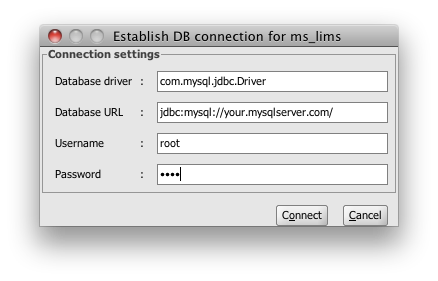
\includegraphics[width=0.80 
	\textwidth]{../Images/connection-empty.png} \centering \label{fig:connection} \caption{The Connection Dialog allows then users to connect to the running MySQL server.} 
\end{figure}

\npar Enter \emph{your.mysqlserver.com} in the Database URL field, then enter your username and password before establishing the database connection by clicking the \textbf{Connect} button. \npar Ok, now ms-lims is connected to the MySQL server, and we have to configure a ms-lims database onto the MySQL server. This can be done by using the \textbf{ConfigurationGUI} that can be started in the menu via \emph{Menu > Database Configuration}. 

\npar Different steps in the ConfigurationGUI are separated in multiple tabs in the top. 
\begin{description}
	\item[summary] Gives an brief overview of the active database. 
	\item[database] Creates the ms-lims relational database scheme into your MySQL database. A relational schema defines a collection of tables, providing structure for the mass spectrometry data that needs to be stored in the database. Just as fragmentation spectra are stored in one table, peptide identifications are stored in different table. Hence, a connection between both tables is maintained. More, both are connected to another table that reflects which instrument was used. As such, you can eventually retrieve all spectra from a given instrument or all peptides containing a particular sequence. 
	\begin{figure}
		[H] 
		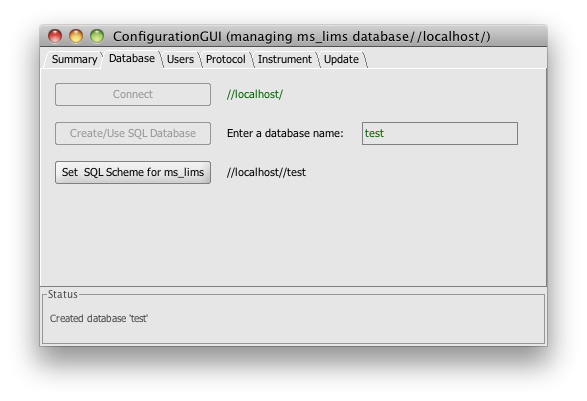
\includegraphics[width=0.80 
		\textwidth]{../Images/config-database.png} \centering \label{fig:config-database} \caption{The database tab in the ConfigurationGUI.} 
	\end{figure}
	\begin{itemize}
		\item \textbf{Connect} to the MySQL database system you previously installed by using the 'root' username and password . Fill in the address of the computer that has the MySQL server running. If the MySQL server is installed on this system, fill in \textbf{'localhost' }to refer to this local computer. Otherwise, fill in the address of the computer within your network. 
		\item \textbf{Create SQL Database} to create a new ms-lims database on the MySQL server. Fill in an appropriate name such as \textbf{'projects' } to as a identifier for the ms-lims database. 
		\item \textbf{Set SQL Scheme for ms-lims} to the (ex.) 'projects' database. 
	\end{itemize}
	Now the database is structured, it is ready to store mass spectrometry data in a relational manner. 
	\item[users] Add or remove ms-lims users from the database system. An ms-lims user can be a mass spectrometrist storing fragmentation spectra or a informatician storing peptide identification results. 
	\begin{figure}
		[H] 
		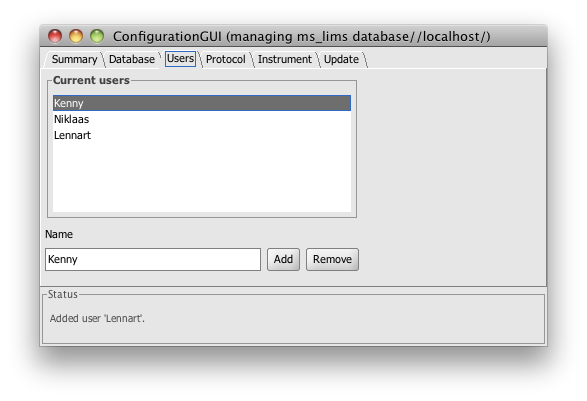
\includegraphics[width=0.80 
		\textwidth]{../Images/config-user.png} \centering \label{fig:config-user} \caption{The user tab in the ConfigurationGUI.} 
	\end{figure}
	
	\item[protocols] Add or remove ms-lims protocols from the database system. 
	\begin{figure}
		[H] 
		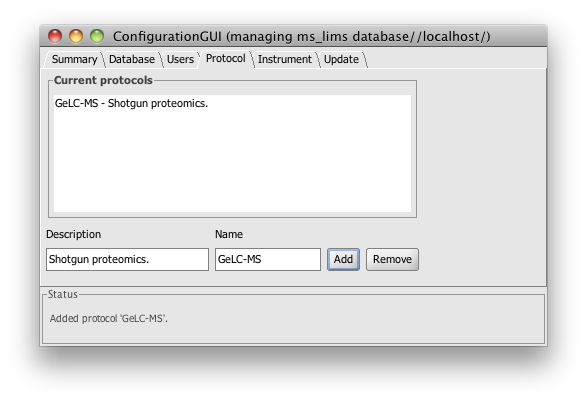
\includegraphics[width=0.80 
		\textwidth]{../Images/config-protocol.png} \centering \label{fig:config-protocol} \caption{The protocol tab in the ConfigurationGUI.} 
	\end{figure}
	
	\item[instrument] Add or remove ms-lims instruments from the database system. ms-lims is independent from mass spectrometer vendors by storing fragmentation spectra in a uniform manner. Hence, as different vendors have different forms of output, .pkl files versus .xml or single versus merged files, ms-lims has different engines to store each fragmentation spectrum as a single entity independent from vendors. In this panel you are ought to define which instrument is used in order to store the data into ms-lims appropriately. \\\textit{If your instrument of choice is not listed, please contact the ms-lims user group at \url{http://groups.google.com/group/ms_lims}} 
	\begin{figure}
		[H] 
		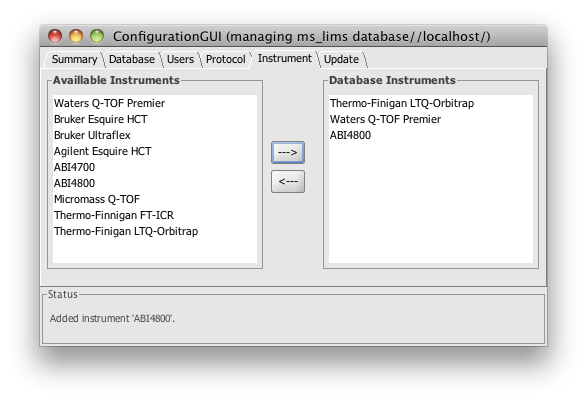
\includegraphics[width=0.80 
		\textwidth]{../Images/config-instrument.png} \centering \label{fig:config-instrument} \caption{The instrument tab in the ConfigurationGUI.} 
	\end{figure}
\end{description}
\npar Ok, the MySQL database is now running a relational database scheme capable for managing proteomics data. Only a few minor steps to go!

\subsection*{Updates} \npar Ms-lims is a continuously growing system and it is required to create new tables in the database schema or modify the existing content in the database. Therefore, we provide \textbf{update scripts} if required and these updates can also be applied in the ConfigurationGUI. Please find the latest update scripts on the ms-lims project site (\url{http://code.google.com/p/ms-lims/wiki/Updates}). 
\begin{figure}
	[H] 
	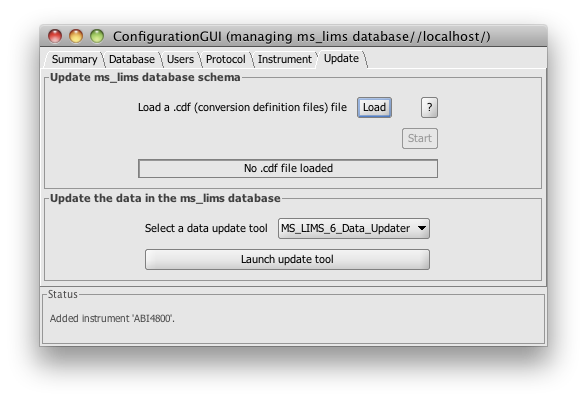
\includegraphics[width=0.80 
	\textwidth]{../Images/config-update.png} \centering \label{fig:config-update} \caption{The update tab in the ConfigurationGUI.} 
\end{figure}

\subsection*{Logs and Properties} \npar The properties and log files are saved to the user's home directory in the \textbf{.compomics/ms-lims/} folder. Two files can be found there: 
\begin{itemize}
	
	\item[mslims-log4j.log] This text file logs all the normal output and the unexpected errors that occur while running ms-lims. If something unexpected occurs, please attach this file while posting the issue on \url{http://code.google.com/p/ms-lims/issues/list}. 
	\item[mslims.properties] This properties file contains startup properties of ms-lims. 
\end{itemize}

\begin{tabular*}{0.80\textwidth}
	{| l | p{0.69\textwidth}|}
\hline
  user &                                                                                                                                                                                       The default username for the database connection.\\
\hline
   url &                                                                                                                                                                                   The default url to the database. (Leave the default!)\\
\hline
driver &                                                                                                                                                         The default java driver to create the database connection. (Leave the default!)\\
\hline
  java & The Java startup parameters. Change \textbf{Xmx...m} to set your preferred amount of memory usage. Xmx1024m would for instance result in 1024MB virtual memory. This parameter should be increased if you receive out of memory errors.\\
\hline
\end{tabular*}

\part{Ms-lims Tools}

% Reset counters for the second part.
\setcounter{chapter}{0} \setcounter{figure}{0}

\chapter{Overview}\label{Overview} \npar After ms-lims has been successfully installed, the end-users can start making use of the client tools that work the database. Some tools serve to insert information in the database, while others assist to extract and interpret the information that has been stored in the database. The hierarchy of the tools is similar to the time course of an experiment. First, a project must be created to encompass all information involved in a single experiment, and this can be done via the ProjectManager tool (\ref{sec:projectmanager}). Second, the MS/MS spectra must be stored in the ms-lims database by the SpectrumStorage tool (\ref{sec:spectrumstorage}), and the MS/MS spectra can be extracted from the database subsequently by MergerGUI (\ref{sec:merger}) for further analysis by external database search engines. Once the Ms/MS spectra interpretation into peptide identifications by Mascot has been completed, the searches can be stored into ms-lims by IdentificationGUI (\ref{sec:identification}). Furthermore, if peptide quantification was performed in parallel by Mascot, then this can be persisted into the database as well by the QuantitationGUI (\ref{sec:quantitation}). Following these storage tools, all information can be further analyzed via standardized project reports of the ProjectAnalyzer tool (\ref{sec:projectanalyzer}) or via custom SQL queries in the GenericQuery tool (\ref{sec:genericquery}). Finally, the results can be validated in depth on the level of peptide identifications by Peptizer (\ref{sec:peptizer}) or peptide quantitations by Rover (\ref{sec:rover}). \\Each of these tools are explained in the following sections.

\npar The appearance of the main GUI for ms-lims is a menu bar and list of buttons. Here you can choose which tool you would like to start. The buttons from up to down follow the workflow which you should meet when working with ms-lims. You can use shortcuts to start the tools, e.g. \texttt{Alt+1} starts the ProjectManager. Just try out the pulldown menu in the menu bar. Now we will take a closer look at the tools. 
\begin{figure}
	[H] 
	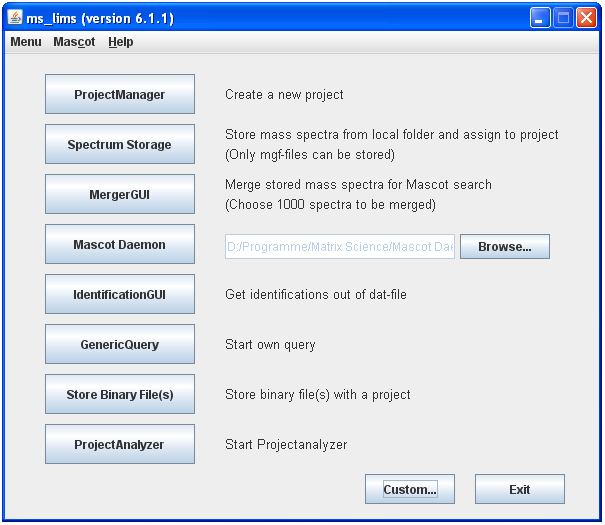
\includegraphics[width=0.80 
	\textwidth]{../Images/startup_mslims2.png} \centering \label{fig:overview} \caption{The ms-lims menu consists of several buttons. Just click on the buttons to start the corresponding tool.} 
\end{figure}

\chapter{Starting ms-lims} The main tools of ms-lims are provided by an application GUI, which can be started by double clicking the ms-lims jar executable file. When you start up ms-lims, the database connection dialog will appear. Enter your username and password here to connect to the ms-lims database.

\chapter{Managing projects by the ProjectManager} \label{sec:projectmanager} The ProjectManager simply organize the projects which you can create or modify here. A project includes the mass spectra and mascot searches of an experiment. To get a better overview of your projects, you can check the box \emph{Sort projects alphabetically}. 
\begin{figure}
	[H] 
	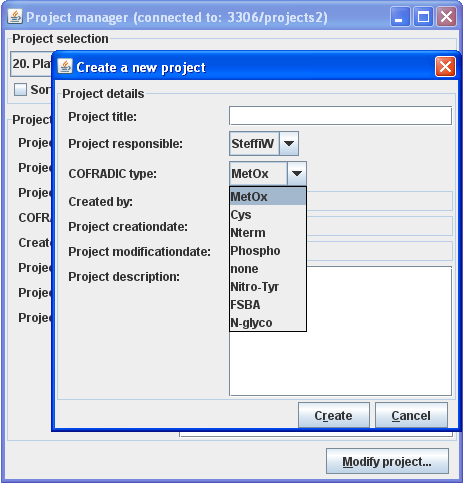
\includegraphics[width=0.80 
	\textwidth]{../Images/manager_newproj.png} \centering \label{fig:projectmanager} \caption{The ProjectManager allows you to create new projects.} 
\end{figure}
To create a new project, click on the button \emph{Create new project}. Enter a meaningful title for your project. In the next steps you will identify your project only by this title. Choose the project responsible person then and select the COFRADIC type if you did a COFRADIC experiment. If you did a other kind of experiment, please select \emph{none} (See figure \ref{fig:projectmanager}). The project description allows you e.g.\ to make a note of the experimental setup of the project. When you have finished select \emph{Create}. A project number will be assigned automatically to your project. If you just want to edit an existing project, click on the button \emph{Modify project}. Don't forget to save the changes on your project. To exit this tool just close the tool window.

\chapter{Storing MS/MS spectra by the SpectrumStorageGUI} \label{sec:spectrumstorage} This tool allows you to store spectra assigned to a project in the database. When you start the tool, there's a dialog where you can choose the mass spectrometer instrument where the spectra were derived from. Please note that the instrument table has to be set up in the database where the correct storage engine class has to be defined for the relevant instrument. 
\begin{figure}
	[H] 
	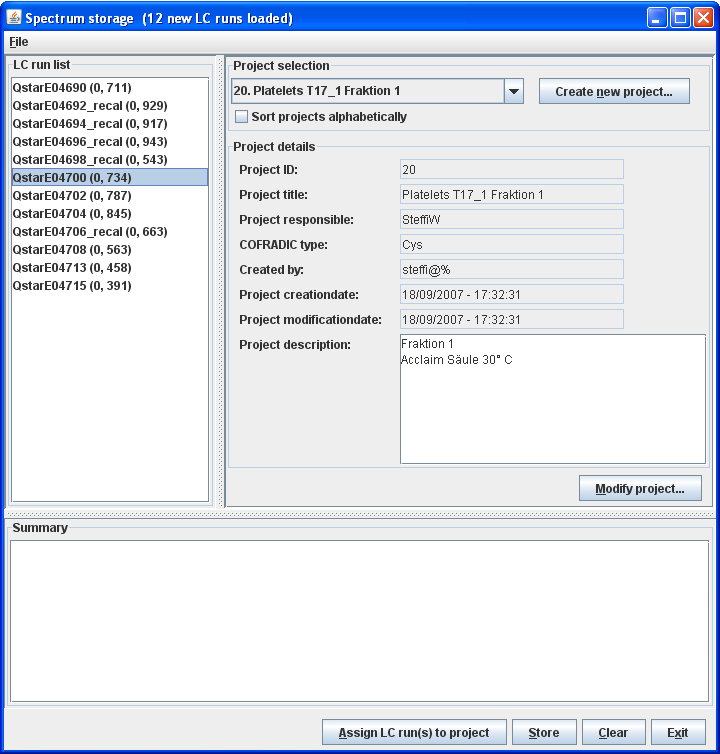
\includegraphics[width=0.80 
	\textwidth]{../Images/spectrum_storage.png} \centering \label{fig:spectra1} \caption{Here you can assign mass spectra to a project and store them in the database.} 
\end{figure}

The window of the SpectrumStorageGUI consists of three parts: left, right and lower window.\\
In the left window (LC run list) you'll see the spectra files you just loaded. By doubleclicking on a file in the LC run list you can add a comment concerning that LC run.\\
Choose the project to which the spectra belong to in the right window \emph{Project selection}. You also can create or modify the project here. Mark all spectra you want to add to the choosen project in the LC run list. Click on the button \emph{Assign LC run(s) to project}. 
\begin{figure}
	[H] 
	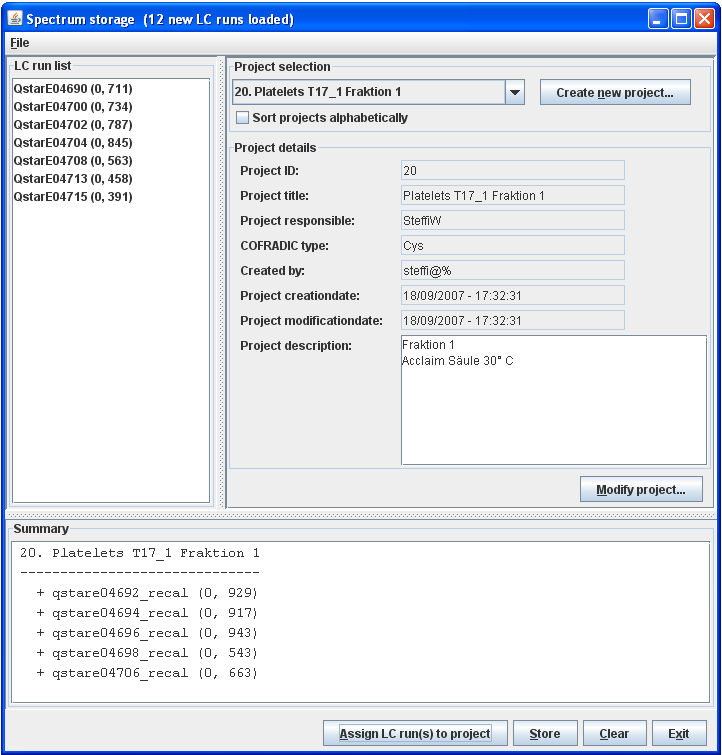
\includegraphics[width=0.80 
	\textwidth]{../Images/spectrum_storage_assign.png} \centering \label{fig:spectra3} \caption{Mark the spectra you want to assign to a project in the upper window.} 
\end{figure}

Then you can check your selection in the lower window \emph{Summary}. By pressing \emph{Clear} the selection is cancelled and can be done again. Finally, to commit the selected spectra to the database click the button \emph{Store}. This process can take a while depending on the size and number of spectra.

\chapter{Extracting MS/MS spectra from ms-lims by the MergerGUI} \label{sec:merger} The job of the MergerGUI is in short, to merge your stored spectra to a set of files before you submit them to the Mascot search engine.\\
\begin{figure}
	[H] 
	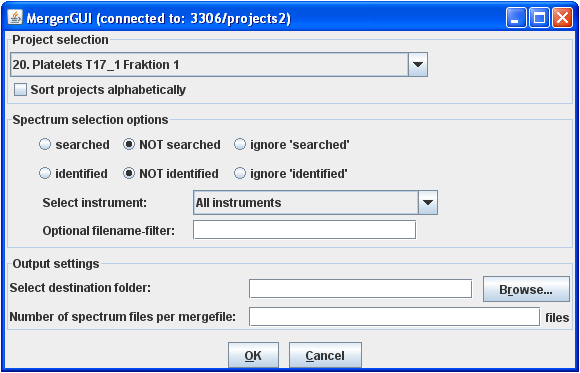
\includegraphics[width=0.80 
	\textwidth]{../Images/merger.png} \centering \label{fig:merger} \caption{The MergerGUI organizes your spectra to a set of files} 
\end{figure}

First choose the project whose spectra you want to be merged. When you merge the files for the first time, do not check the spectrum select options \emph {NOT searched}, \emph {NOT identified} in the section \emph {Spectrum file options}. In the next step, select your instrument where the spectrafiles have been derived from and optional, choose a file filtername if a limit selection of files is needed, e.g. 'LTQ003*'. In the section \emph {Output settings} pick or create a folder where the merged files can be stored. Enter the number of spectra files you want to be merged. A good starting point is a value of 1000 files. 

%% Anyway this is a Mascot search property, explain further
The next time if you want to redo a search, check the spectrum select options \emph {searched} and \emph {NOT identified} to get a subset of the spectra which need fitted search parameters for identification for example.

\chapter{Identifying MS/MS spectra by Mascot Daemon} \label{sec:mascotdaemon} Up to now, ms-lims can only process datafiles from the Mascot search engine.

%% Building up the ODBC coupling to the Mascot task database
%% Coming up OMSSA interface??
This button will start your MascotDaemon application. You can store the local path to the MascotDaemon application permanently in the mascotdaemon.properties file like 
\begin{verbatim}
	MASCOTDAEMONFILE= 
\end{verbatim}
\par 
\begin{verbatim}
	C:/Program files/Matrix Science/Mascot Daemon/Daemon.exe 
\end{verbatim}
or enter the path directly in the field beside the button.\\
Now select the merged files for searching with Mascot you have created before with the MergerGUI tool. Then start your Mascot search as usual. It is important to use the merged files for searching and not the original spectra files at this point, otherwise ms-lims will prompt an error message. The merged files are connected to the database and to your project. 

\chapter{Storing peptide identifications by the IdentificationGUI} \label{sec:identification} This tool allows you to parse and view your Mascot search results directly from the Mascot dat files and finally store them in the database. IdentificationGUI connects with your task database from MascotDaemon. Each time IdentificationGUI is started, you have to show ms-lims where to find this \textbf{TaskDB.mdb} file that lists your Mascot Searches and is typically stored in your Mascot Daemon installation folder. A list with your actual Mascot searches will subsequently appear, with the last Mascot search task displayed in the top. Here you select the results you want to parse. Click on the nodes to see which files belong to you search. Select one or multiple searches from the tree list, then mark your desired result file(s) in the right window. The identity threshold score applied for the extraction of the selected files can be set at the bottom of the window. The default is set at the Mascot standard 95\% confidence which allows a maximum of 5\% false positive identifications. 
\begin{figure}
	[H] 
	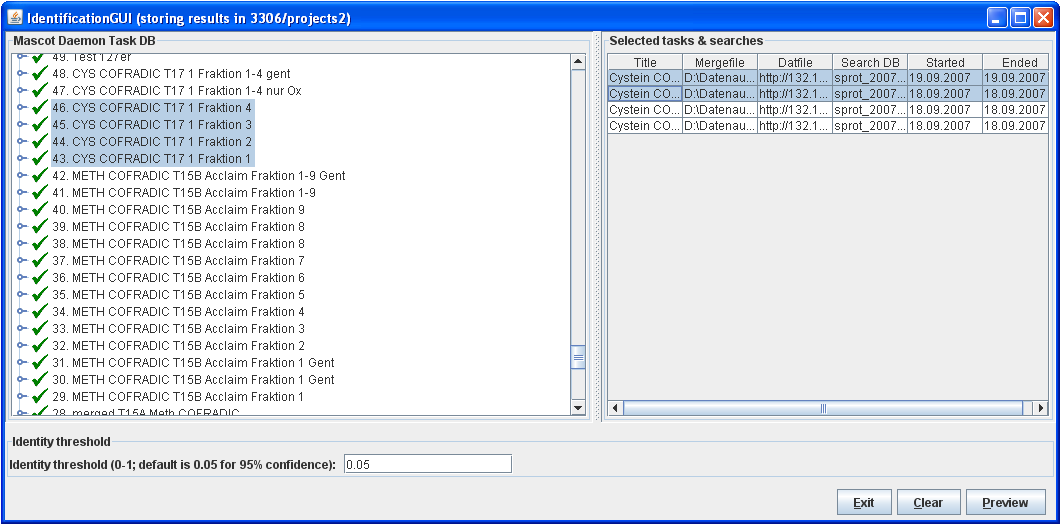
\includegraphics[width=0.80 
	\textwidth]{../Images/identification.png} \centering \label{fig:identification} \caption{Choose the Mascot searches you want to parse} 
\end{figure}
By selecting the \emph{Preview} button the tool will start to retrieve the results and parse them. The proceeding is indicated by a progressbar and according to the file size this task can take a while. When the parsing of the results has finished, a table is displayed which contains the identified peak list from the selected search. 
\begin{figure}
	[H] 
	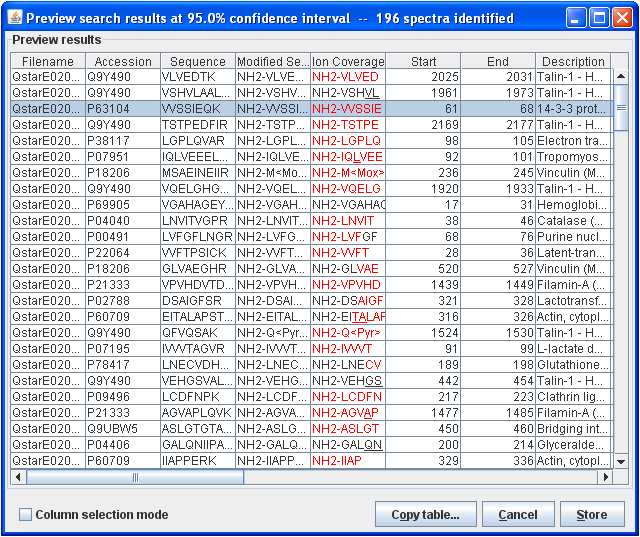
\includegraphics[width=0.80 
	\textwidth]{../Images/preview.png} \centering \label{fig:identificationpreview} \caption{The Preview table shows a list of all identified peptides of the selected search} 
\end{figure}
Here you can simply copy and paste the results to other applications as spreadsheet for example. {\emph{Hint:} Of course you can use the IdentificationGUI tool just to parse your Mascot searches without storing them to the database.} You can adjust this preview table to your requirements and sort a certain column (descending or ascending), resize or move a column. If the \emph{Column selection mode} is checked you can mark columns for copy and paste instead of marking the rows as normally. The columns in the preview table presents following data: 
\begin{description}
	\item [Filename] Refers to the original filename the spectra came from. Sometimes also some spectra header information can be seen here 
	\item [Accession] The protein accession as received from the search database. A left mouse button double click opens the entry the UniPro database 
	\item [Sequence] The peptide sequence as received from the search database 
	\item [Modified sequence] The peptide sequence is supplemented with the fixed or variable modifications if they occur. Note: a star marks the modification as fixed e.g. (Cmm*) 
	\item [Ion Coverage] Highlights the ionseries; for y-ions: red font color, for b-ions: underlined 
	\item [Start/End] Start/End of the peptide within the protein sequence 
	\item [Description] The description as received from the search database 
	\item [Title] Refers to the search title in mascot 
	\item [Score/Threshold] Refers to the score/threshold from mascot 
	\item [Confidence] As set in IdentificationGUI before parsing 
	\item [Calculated/Experimental mass] Refers to the calculated/experimental mass from mascot 
	\item [Isoforms] Lists isoforms to that peptide 
	\item [Precursor (m/z)] The precursor mass of that peptide 
	\item [Charge] The charge of that peptide 
	\item [Enzymatic] Refers to the enzyme cleavage state: FE - correct enzymatic cleavage; NE - n-terminal correct; CE - c-terminal correct; EE - fully incorrect 
	\item [Datfile] The name of datfile which has been generated on this search 
	\item [Search database filename] Exact filename of the search database 
	\item [Search DB] Name of the search database 
\end{description}
If you decided that the data in the preview table can be stored in the database, just press the \emph{Store} button. Again you will see a progressbar and finally a small box informing you that all identifications have been stored in the database.

\chapter{Storing peptide quantitations by the QuantiationGUI} \label{sec:quantitation} \npar Similar to the IdentificationGUI tool, the QuantitationGUI tool will first process all peptide quantitations associated with a set of peptide identifications from a Mascot search. If the peptide identifications are successfully mapped to peptide quantitations, then they are previewed prior to the final storage into the database.

\chapter{Retrieving information from the database by custom SQL queries in the GenericQuery tool} \label{sec:genericquery} GenericQuery allows you to do queries within your database using SQL (Structured Query Language). This feature is for advanced users, because you need a basic knowledge about how to perform a SQL query. 
\begin{figure}
	[H] 
	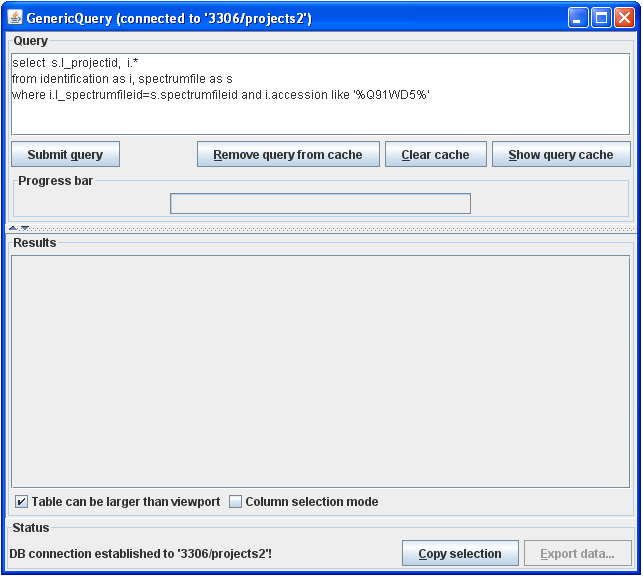
\includegraphics[width=0.80 
	\textwidth]{../Images/genericquery.png} \centering \label{fig:genericquery} \caption{The GenericQueryGUI allows access to all tables and stored data by using SQL} 
\end{figure}
In the upper window you can type your query and submit it. Don't forget to connect to your database first (use projects e.g.). All submitted queries are stored in cache, so you can access recent queries (up to 40 entries). The lower window will show your result table, which one can simply copy and paste to spreadsheet applications or export the data in .html or .csv format. 
\begin{figure}
	[H] 
	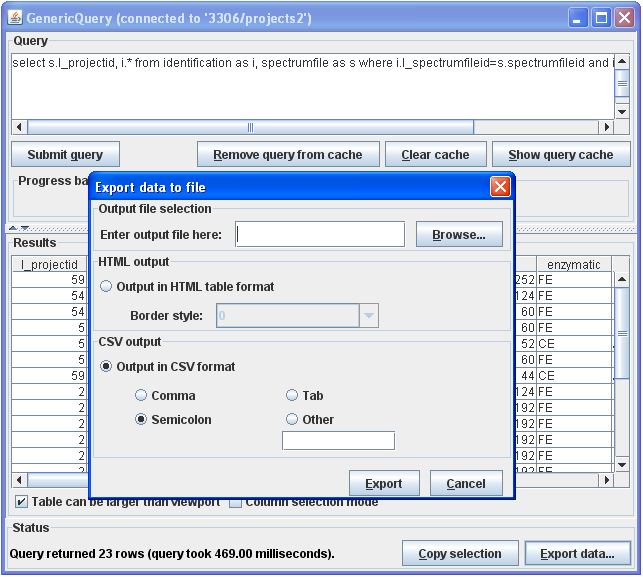
\includegraphics[width=0.80 
	\textwidth]{../Images/genericquery2.png} \centering \label{fig:genericquery_export} \caption{The GenericQueryGUI allows access to all tables and stored data by using SQL} 
\end{figure}
Some useful queries for proposal are listed below:\\
\textbf{select * from project where username like 'myname\%'} - List all my projects\\
\textbf{select s.l\_projectid, i.* from identification as i, spectrumfile as s\\
where i.l\_spectrumfileid=s.spectrumfileid and i.accession like '\%myAccession\%'} - List only projects and identifications where that protein accession has been identified

\chapter{Retrieving standardized reports from the database by the ProjectAnalyzer tool} \label{sec:projectanalyzer} The ProjectAnalyzer tool provides a set of three tools for the data analysis to be performed on a selected project: \emph{Binary file retriever tool}, \emph{DescriptiveNumbersTool} and \emph{Descriptive numbers tool}. Just select the tools from the drop-down menu. 
\begin{figure}
	[H] 
	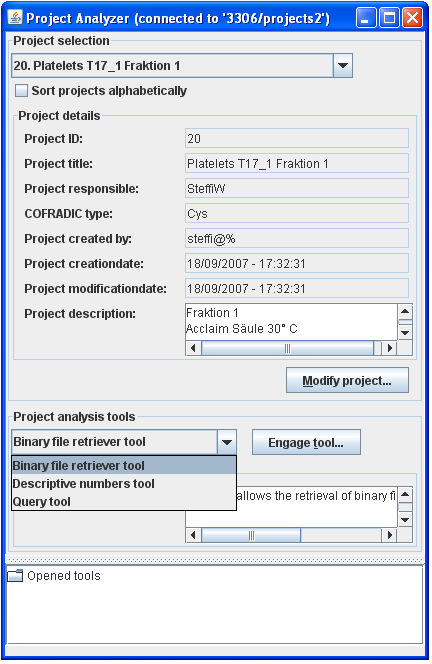
\includegraphics[width=0.80 
	\textwidth]{../Images/project_analyzer.png} \centering \label{fig:project_analyzer} \caption{Three tools to analyze your projects} 
\end{figure}

\section{Storing and retrieving Binary file(s) into ms-lims}

\npar Use this tool to append an informative protocol, image or text-file to a project. Define a descriptor as you like which specifies the binary file e.g. as text document, spreadsheet or picture. 
\begin{figure}
	[H] 
	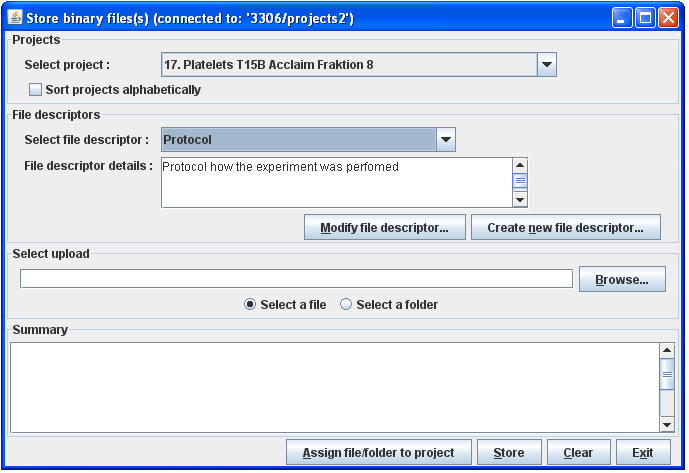
\includegraphics[width=0.80 
	\textwidth]{../Images/binary_file.png} \centering \label{binary_file} \caption{Assign a binary file to your project} 
\end{figure}

\npar To locate a binary file stored with a project, run the binary file retriever tool. Select your project in the upper window and then run the tool by hitting \emph{Engage tool}. There'll be pop up a dialog where you can select the binary file and save it to any destination.

\section{Descriptive numbers tool} This tool gives a result overview for COFRADIC experiments. If the experiment COFRADIC type \textit{N-term}, \textit{MetOx} or \textit{Cys} has been selected when creating the project, this tool calculates some informative numbers. Some SQL queries will be performed then and generating the report therefore can take a while. A statusbar will inform you about the progress. The final report can be simply copied and pasted to any document.

\section{Query tool} Here you can run a set of predefined SQL queries against the selected project. This option is very useful for beginners to start with analyzing the stored data. The queries are: 
\begin{figure}
	[H] 
	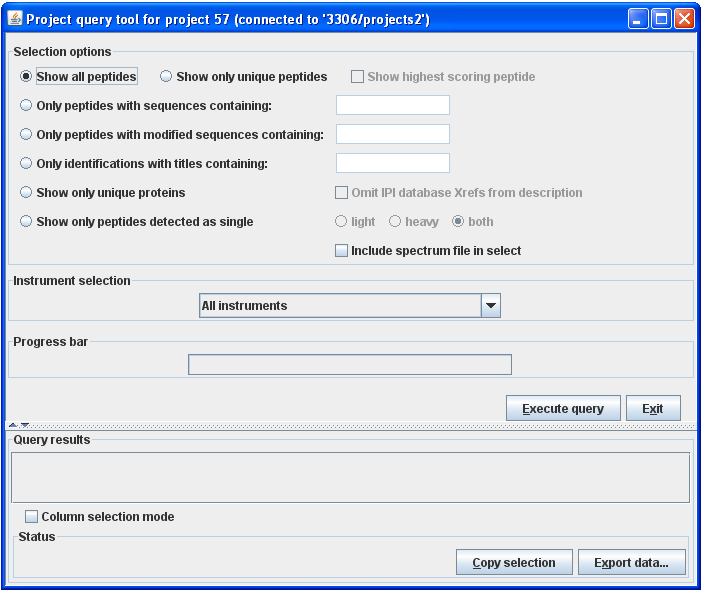
\includegraphics[width=0.80 
	\textwidth]{../Images/querytool.png} \centering \label{querytool} \caption{Query tool with predefined SQL queries} 
\end{figure}
\begin{description}
	\item [Show all identified peptides] Simply list all identified peptides 
	\item [Show only unique peptides] Check the box if only unique peptides with the maximun score should be displayed 
	\item [Only peptides with sequences containing] Enter a searchstring use '\%' as wildcard(s) 
	\item [Only peptides with modified sequences containing] Enter a searchstring; use '\%' as wildcard(s) 
	\item [Only identifications with title containing] Enter a searchstring; use '\%' as wildcard(s) 
	\item [Show only unique proteins] A list of all unique proteins - you can omit the appearance of cross references from the IPI database 
	\item [Show only peptides detected as single] Choose light, heavy or both kind of peptides 
\end{description}
When you have selected a query, choose the instrument if required and press \emph{Execute query}. It's useful to enable the checkbox \emph{Include spectrumfile in select} so a spectrum viewer application opens when you right-click on a spectrumfile in the result table. Again, you can simply copy and past the results to a spreadsheet or export the data as explained in chapter \ref{sec:genericquery}. 
\begin{figure}
	[H] 
	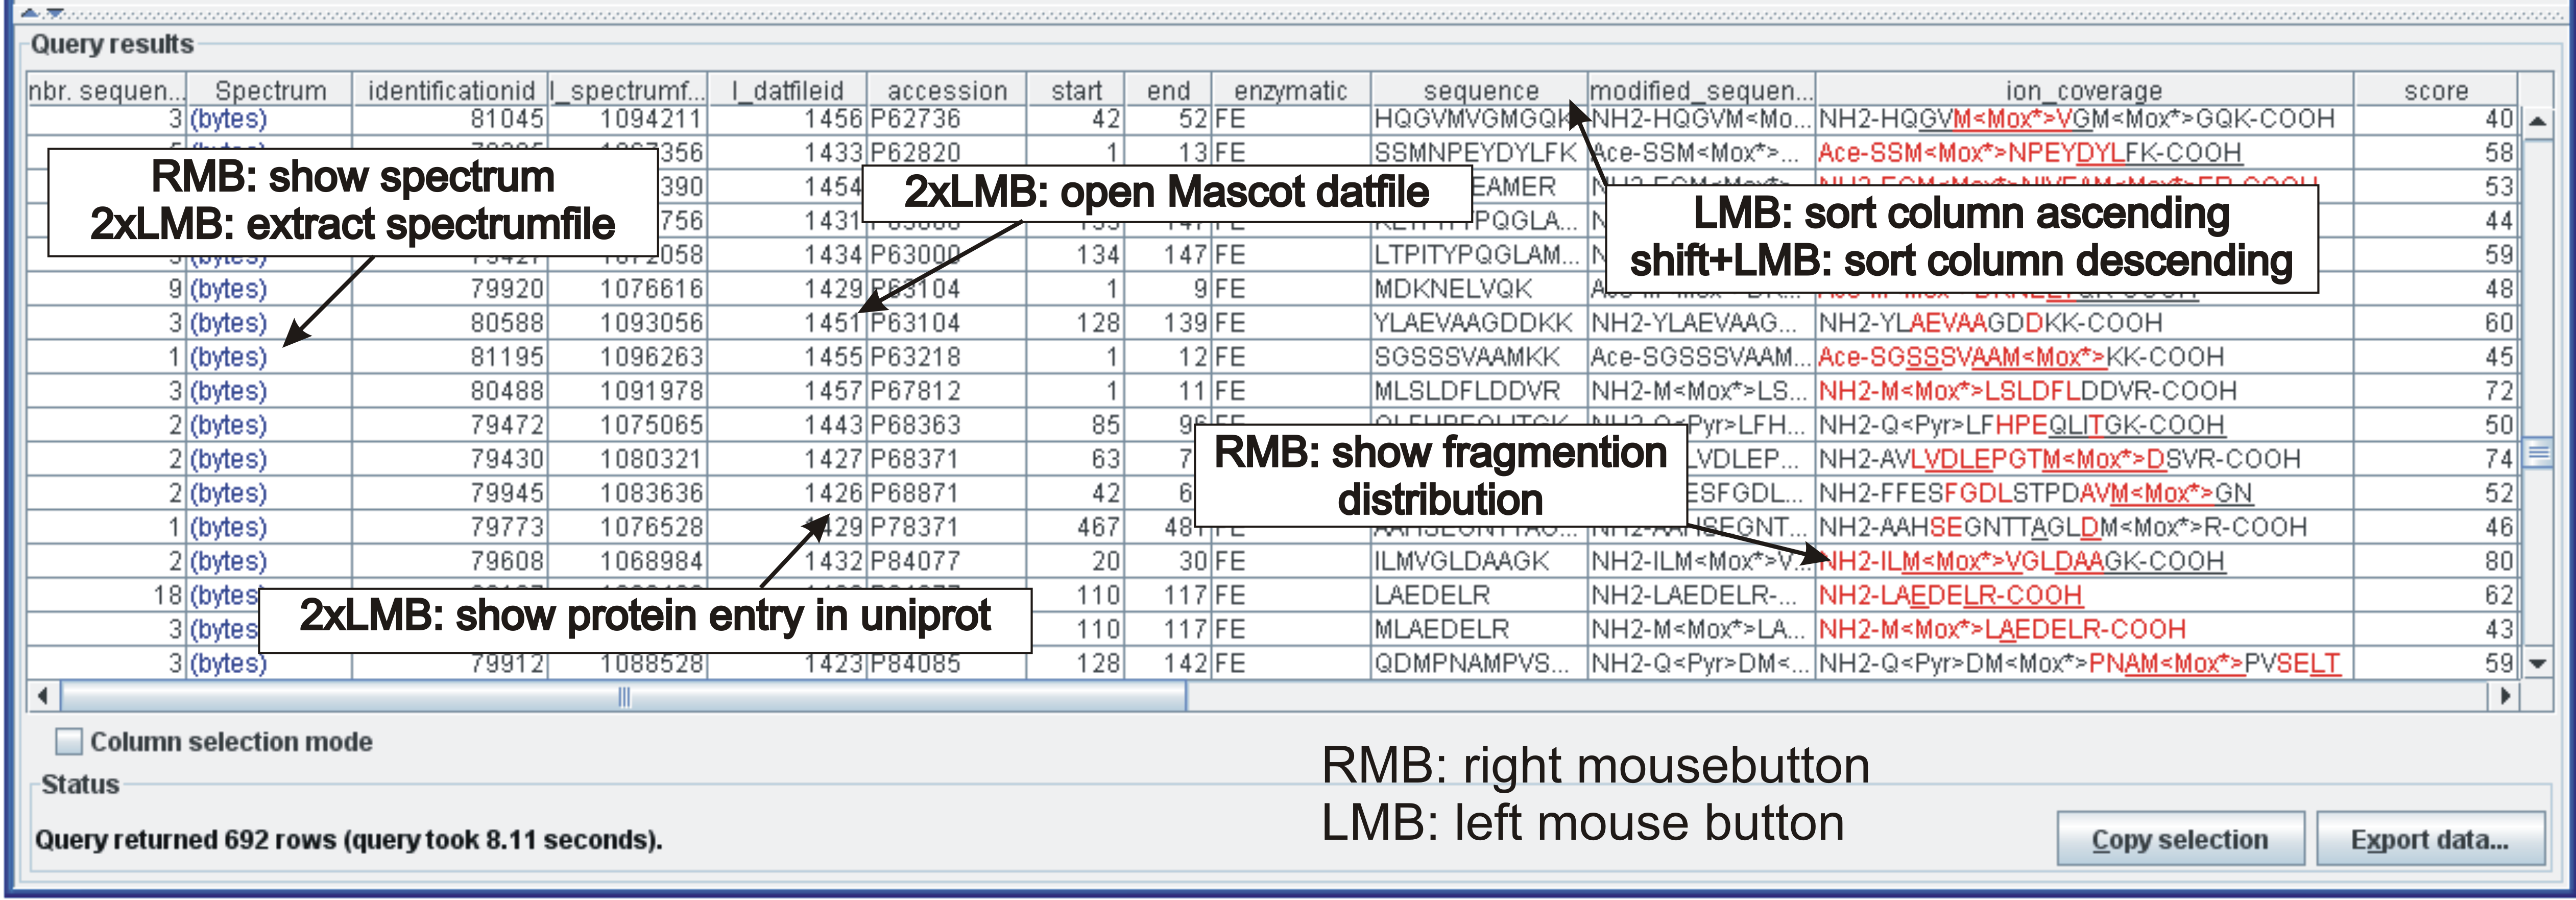
\includegraphics[width=0.80 
	\textwidth]{../Images/results_ext.png} \centering \label{fig:resulttable} \caption{The results table allows interactive exploration features} 
\end{figure}

\chapter{Validating peptide identifications by Peptizer} \label{sec:peptizer} \npar For manual validation of peptide identifications, ms-lims joins forces with the Peptizer tool. Peptizer supplies a platform allowing you to easily create an automated expert system to assure the quality of the peptide identifications. \\The integration of ms-lims and peptizer is two-sided: Peptizer can inspect peptide identifications by their ms-lims derived identificationID, or by their association to a specific ms-lims project; and, when validation has been performed - the results can be persisted into ms-lims as well.

For more information on Peptizer, please visit \href{http://peptizer.googlecode.com}{the peptizer project site}.

\chapter{Validating peptide quantitation by Rover} \label{sec:rover} \npar For manual validation of peptide identifications, ms-lims joins forces with the Rover tool. Rover supplies a platform allowing you to easily filter the relevant outliers in your quantitative experiment. Furthermore, Rover provides an of quality related attributes in a protein centric view and thereby enables an optimal judgement on the reliability of the resulting peptide quantitation. 

For more information on Rover, please visit \href{http://compomics-rover.googlecode.com}{the rover project site}.

\end{document} 
